\documentclass[]{elsarticle} %review=doublespace preprint=single 5p=2 column
%%% Begin My package additions %%%%%%%%%%%%%%%%%%%
\usepackage[hyphens]{url}
\usepackage{lineno} % add
\providecommand{\tightlist}{%
  \setlength{\itemsep}{0pt}\setlength{\parskip}{0pt}}

\bibliographystyle{elsarticle-harv}
\biboptions{sort&compress} % For natbib
\usepackage{graphicx}
\usepackage{booktabs} % book-quality tables
%% Redefines the elsarticle footer
%\makeatletter
%\def\ps@pprintTitle{%
% \let\@oddhead\@empty
% \let\@evenhead\@empty
% \def\@oddfoot{\it \hfill\today}%
% \let\@evenfoot\@oddfoot}
%\makeatother

% A modified page layout
\textwidth 6.75in
\oddsidemargin -0.15in
\evensidemargin -0.15in
\textheight 9in
\topmargin -0.5in
%%%%%%%%%%%%%%%% end my additions to header

\usepackage[T1]{fontenc}
\usepackage{lmodern}
\usepackage{amssymb,amsmath}
\usepackage{ifxetex,ifluatex}
\usepackage{fixltx2e} % provides \textsubscript
% use upquote if available, for straight quotes in verbatim environments
\IfFileExists{upquote.sty}{\usepackage{upquote}}{}
\ifnum 0\ifxetex 1\fi\ifluatex 1\fi=0 % if pdftex
  \usepackage[utf8]{inputenc}
\else % if luatex or xelatex
  \usepackage{fontspec}
  \ifxetex
    \usepackage{xltxtra,xunicode}
  \fi
  \defaultfontfeatures{Mapping=tex-text,Scale=MatchLowercase}
  \newcommand{\euro}{€}
\fi
% use microtype if available
\IfFileExists{microtype.sty}{\usepackage{microtype}}{}
\usepackage{longtable}
\usepackage{graphicx}
% We will generate all images so they have a width \maxwidth. This means
% that they will get their normal width if they fit onto the page, but
% are scaled down if they would overflow the margins.
\makeatletter
\def\maxwidth{\ifdim\Gin@nat@width>\linewidth\linewidth
\else\Gin@nat@width\fi}
\makeatother
\let\Oldincludegraphics\includegraphics
\renewcommand{\includegraphics}[1]{\Oldincludegraphics[width=\maxwidth]{#1}}
\ifxetex
  \usepackage[setpagesize=false, % page size defined by xetex
              unicode=false, % unicode breaks when used with xetex
              xetex]{hyperref}
\else
  \usepackage[unicode=true]{hyperref}
\fi
\hypersetup{breaklinks=true,
            bookmarks=true,
            pdfauthor={},
            pdftitle={A simplified dynamic bioenergetic model for coral-Symbiodinium symbioses},
            colorlinks=true,
            urlcolor=blue,
            linkcolor=magenta,
            pdfborder={0 0 0}}
\urlstyle{same}  % don't use monospace font for urls
\setlength{\parindent}{0pt}
\setlength{\parskip}{6pt plus 2pt minus 1pt}
\setlength{\emergencystretch}{3em}  % prevent overfull lines
\setcounter{secnumdepth}{0}
% Pandoc toggle for numbering sections (defaults to be off)
\setcounter{secnumdepth}{0}
% Pandoc header


\usepackage[nomarkers]{endfloat}

\begin{document}
\begin{frontmatter}

  \title{A simplified dynamic bioenergetic model for coral-\emph{Symbiodinium}
symbioses}
    \author[University of Hawaii]{Ross Cunning\corref{c1}}
   \ead{ross.cunning@gmail.com} 
   \cortext[c1]{Corresponding Author}
    \author[University of California]{Erik B. Muller}
  
  
    \author[University of Hawaii]{Ruth D. Gates}
  
  
    \author[University of California]{Roger M. Nisbet}
  
  
      \address[University of Hawaii]{Hawaii Institute of Marine Biology, Kaneohe, HI 96744, USA}
    \address[University of California]{Department of Ecology, Evolution, and Marine Biology, Santa Barbara, CA
93106, USA}
  
  \begin{abstract}
  This is the abstract.
  \end{abstract}
  
 \end{frontmatter}

\section{Introduction}\label{introduction}

The nutritional exchange between corals and \emph{Symbiodinium} directly
underlies the capacity of corals to build coral reef ecosystems, worth
trillions of US Dollars annually (Costanza, Groot, and Sutton 2014).
However, the complex symbiotic metabolism of corals is vulnerable to
disruption by numerous anthropogenic environmental perturbations,
jeopardizing their future persistence. In order to understand and
predict coral responses to complex changes in the environment, a
mechanistic understanding of how multiple interacting factors drive the
individual and emergent physiology of both symbiotic partners is
necessary. Such a task is well suited for theoretical modeling
frameworks such as Dynamic Energy Budget (DEB) theory (Kooijman 2010),
although the complexity of such theory makes these efforts inaccessible
to many biologists (Jager, Martin, and Zimmer 2013). In order to bridge
this gap, we present here a simplified dynamic bioenergetic model for
coral-\emph{Symbiodinium} symbioses that aims to mechanistically
integrate the impacts of complex environmental change on the
physiological ecology of reef corals.

In reef coral symbioses, intracellular \emph{Symbiodinium} translocate
photosynthetically-fixed carbon to support coral metabolism, and utilize
the animal's metabolic waste products, including nitrogenous compounds
and carbon dioxide, in return (Muscatine and Porter 1977). Previous
application of DEB theory to this syntrophic system (Muller et al. 2009)
demonstrated a stable symbiotic relationship and qualitatively realistic
growth and biomass ratios across gradients of ambient irradiance,
nutrients, and food. This model assumed that 1) \emph{Symbiodinium} has
priority access to carbon through photosynthesis, 2) the coral animal
has priority access to dissolved nitrogen through contact with seawater,
and 3) each partner shares with the other only what it cannot use
itself. In its simplest form, this principle of sharing the surplus
sufficiently describes diverse syntrophic interactions among organs and
organisms (e.g., trees, duckweeds, corals), suggesting the mechanism is
mathematically and evolutionarily robust (Nisbet et al., submitted).

While the work of Muller et al. (2009) applying DEB formalism to this
system represents the most significant theoretical contribution in coral
symbiosis research to date, we aim to strengthen the role of theory and
broaden its potential application to corals in three primary ways:

\begin{enumerate}
\def\labelenumi{\arabic{enumi}.}
\item
  \emph{Develop a detailed module of environmental stress.} Of primary
  interest to coral biologists and ecologists is symbiosis dysfunction
  under environmental stress, resulting in coral ``bleaching''--the loss
  of algal symbionts from the association (Jokiel and Coles 1977).
  Photooxidative stress in \emph{Symbiodinium} is considered a primary
  trigger of bleaching in response to high temperature and/or light
  (Weis 2008), and prolonged or severe bleaching can result in
  mortality, though corals sometimes recover their symbionts. Bleaching
  susceptibility, severity, and recovery may by influenced by
  interacting factors such as heterotrophy and nutrient availability
  (Wooldridge 2014b), and the genetic identity of \emph{Symbiodinium}
  (Glynn et al. 2001). To simulate these bleaching-related phenomena, we
  develop a generalized framework linking overreduction of the
  photosynthetic light reactions to downstream impacts of
  photoinhibition and photodamage.
\item
  \emph{Reduce theoretical and mathematical complexity.} Following the
  logic of Jager, Martin, and Zimmer (2013), we exclude certain features
  of formal DEB models in order to capture behaviors of interest with
  the simplest possible formulation. Here, we present a model without
  reserves, maturity, or reproduction (see Kooijman 2010). This
  formulation restricts the model's scope to the bioenergetics of growth
  and symbiosis dynamics in adult corals, but greatly reduces
  theoretical complexity and parameter numbers, which is advantageous
  given the relative paucity of data for corals. However, our primary
  motivation for reducing complexity was to increase accessibility and
  applicability for biologists and ecologists without requiring
  significant expertise in DEB theory.
\item
  \emph{Provide well-documented, open-access code.} In order to
  facilitate the continued development and application of theoretical
  modeling tools for coral symbioses, we provide open access to the
  model in the form of detailed, commented code written in the R
  language (R Core Team 2014). With an accessible and modular framework,
  we envision this as a resource for futher development by the
  scientific community to include additional complexity and
  problem-specific components. The R language was chosen because it is
  freely available and in common use by biologists and ecologists, to
  widen the audience for this work.
\end{enumerate}

With these as our primary motivations, we describe a simplified approach
to dynamic bioenergetic modeling of coral-algal symbioses that tracks
carbon and nitrogen acquisition and sharing between partners. This
theoretical framework dynamically integrates the influence of external
irradiance, nutrients, and prey availability on coral growth and
symbiosis dynamics (i.e., symbiont:host biomass ratios), allowing for
the possibility of coral bleaching in the event of photooxidative
stress. In the following sections, we describe the formulation of this
model and justify its structure and parameter values based on relevant
literature. We then demonstrate the model's behavior and discuss some of
its major implications and outcomes, and the wide range of potential
applications for this model in the study of cnidarian-algal symbioses.

\section{Model description}\label{model-description}

In this model of coral-algal symbiosis, carbon and nitrogen are acquired
by each partner and used to construct biomass. A graphical
representation of the model is presented in Fig. 1. We use C-moles as
the unit of biomass for consistency with the rigorous mass balance of
DEB theory: 1 C-mole is equivalent to the amount of biomass containing 1
mole of Carbon atoms. Host biomass (\(H\)), symbiont biomass (\(S\)),
and prey biomass (\(X\)) have fixed, but different, molar N:C ratios
(Table 1). Carbon and nitrogen are combined to produce biomass by
synthesizing units (SU), which are mathematical specifications of the
formation of a product from two substrates; we use the ``parallel
complementary'' formulation of Kooijman (2010) to specify these fluxes.
The two state variables in this dynamical system are symbiont biomass
and coral biomass; because resources are acquired proportionally to
surface area (and surface area is assumed proportional to volume for
corals (i.e., they are ``V1-morphs'' in DEB terminology (Kooijman
2010))), biomass increases exponentially during growth. The rate of
increase in coral biomass (i.e.~growth) and the ratio of symbiont to
host biomass are the (i.e.~symbiosis dynamics) are the responses of
interest of the system. Below we describe the formulation of each flux
involved in producing these responses.

Table 1

\begin{longtable}[c]{@{}llll@{}}
\toprule
\begin{minipage}[b]{0.10\columnwidth}\raggedright\strut
Symbol
\strut\end{minipage} &
\begin{minipage}[b]{0.48\columnwidth}\raggedright\strut
Description
\strut\end{minipage} &
\begin{minipage}[b]{0.09\columnwidth}\raggedright\strut
Value
\strut\end{minipage} &
\begin{minipage}[b]{0.23\columnwidth}\raggedright\strut
Units
\strut\end{minipage}\tabularnewline
\midrule
\endhead
\begin{minipage}[t]{0.10\columnwidth}\raggedright\strut
\(n_{NH}\)
\strut\end{minipage} &
\begin{minipage}[t]{0.48\columnwidth}\raggedright\strut
N:C molar ratio in host biomass
\strut\end{minipage} &
\begin{minipage}[t]{0.09\columnwidth}\raggedright\strut
0.19
\strut\end{minipage} &
\begin{minipage}[t]{0.23\columnwidth}\raggedright\strut
--
\strut\end{minipage}\tabularnewline
\begin{minipage}[t]{0.10\columnwidth}\raggedright\strut
\(n_{NS}\)
\strut\end{minipage} &
\begin{minipage}[t]{0.48\columnwidth}\raggedright\strut
N:C molar ratio in symbiont biomass
\strut\end{minipage} &
\begin{minipage}[t]{0.09\columnwidth}\raggedright\strut
0.2
\strut\end{minipage} &
\begin{minipage}[t]{0.23\columnwidth}\raggedright\strut
--
\strut\end{minipage}\tabularnewline
\begin{minipage}[t]{0.10\columnwidth}\raggedright\strut
\(n_{NX}\)
\strut\end{minipage} &
\begin{minipage}[t]{0.48\columnwidth}\raggedright\strut
N:C molar ratio in prey biomass
\strut\end{minipage} &
\begin{minipage}[t]{0.09\columnwidth}\raggedright\strut
0.13
\strut\end{minipage} &
\begin{minipage}[t]{0.23\columnwidth}\raggedright\strut
--
\strut\end{minipage}\tabularnewline
\begin{minipage}[t]{0.10\columnwidth}\raggedright\strut
\(j_{HT}^0\)
\strut\end{minipage} &
\begin{minipage}[t]{0.48\columnwidth}\raggedright\strut
Specific turnover rate of host biomass
\strut\end{minipage} &
\begin{minipage}[t]{0.09\columnwidth}\raggedright\strut
0.03
\strut\end{minipage} &
\begin{minipage}[t]{0.23\columnwidth}\raggedright\strut
\(d^{-1}\)
\strut\end{minipage}\tabularnewline
\begin{minipage}[t]{0.10\columnwidth}\raggedright\strut
\(j_{ST}^0\)
\strut\end{minipage} &
\begin{minipage}[t]{0.48\columnwidth}\raggedright\strut
Specific turnover rate of symbiont biomass
\strut\end{minipage} &
\begin{minipage}[t]{0.09\columnwidth}\raggedright\strut
0.03
\strut\end{minipage} &
\begin{minipage}[t]{0.23\columnwidth}\raggedright\strut
\(d^{-1}\)
\strut\end{minipage}\tabularnewline
\begin{minipage}[t]{0.10\columnwidth}\raggedright\strut
\(\sigma_{NH}\)
\strut\end{minipage} &
\begin{minipage}[t]{0.48\columnwidth}\raggedright\strut
Proportion host nitrogen turnover recycled
\strut\end{minipage} &
\begin{minipage}[t]{0.09\columnwidth}\raggedright\strut
0.9
\strut\end{minipage} &
\begin{minipage}[t]{0.23\columnwidth}\raggedright\strut
--
\strut\end{minipage}\tabularnewline
\begin{minipage}[t]{0.10\columnwidth}\raggedright\strut
\(\sigma_{CH}\)
\strut\end{minipage} &
\begin{minipage}[t]{0.48\columnwidth}\raggedright\strut
Proportion host carbon turnover recycled
\strut\end{minipage} &
\begin{minipage}[t]{0.09\columnwidth}\raggedright\strut
0.9
\strut\end{minipage} &
\begin{minipage}[t]{0.23\columnwidth}\raggedright\strut
--
\strut\end{minipage}\tabularnewline
\begin{minipage}[t]{0.10\columnwidth}\raggedright\strut
\(\sigma_{NS}\)
\strut\end{minipage} &
\begin{minipage}[t]{0.48\columnwidth}\raggedright\strut
Proportion symbiont nitrogen turnover recycled
\strut\end{minipage} &
\begin{minipage}[t]{0.09\columnwidth}\raggedright\strut
0.9
\strut\end{minipage} &
\begin{minipage}[t]{0.23\columnwidth}\raggedright\strut
--
\strut\end{minipage}\tabularnewline
\begin{minipage}[t]{0.10\columnwidth}\raggedright\strut
\(\sigma_{CS}\)
\strut\end{minipage} &
\begin{minipage}[t]{0.48\columnwidth}\raggedright\strut
Proportion symbiont carbon turnover recycled
\strut\end{minipage} &
\begin{minipage}[t]{0.09\columnwidth}\raggedright\strut
0.9
\strut\end{minipage} &
\begin{minipage}[t]{0.23\columnwidth}\raggedright\strut
--
\strut\end{minipage}\tabularnewline
\begin{minipage}[t]{0.10\columnwidth}\raggedright\strut
\(j_{Xm}\)
\strut\end{minipage} &
\begin{minipage}[t]{0.48\columnwidth}\raggedright\strut
Maximum specific feeding rate of host
\strut\end{minipage} &
\begin{minipage}[t]{0.09\columnwidth}\raggedright\strut
0.1292
\strut\end{minipage} &
\begin{minipage}[t]{0.23\columnwidth}\raggedright\strut
\(molX \cdot CmolH^{-1} \cdot d^{-1}\)
\strut\end{minipage}\tabularnewline
\begin{minipage}[t]{0.10\columnwidth}\raggedright\strut
\(K_X\)
\strut\end{minipage} &
\begin{minipage}[t]{0.48\columnwidth}\raggedright\strut
Half-saturation constant for prey uptake by host
\strut\end{minipage} &
\begin{minipage}[t]{0.09\columnwidth}\raggedright\strut
20e-6
\strut\end{minipage} &
\begin{minipage}[t]{0.23\columnwidth}\raggedright\strut
\(molX \cdot L^{-1}\)
\strut\end{minipage}\tabularnewline
\begin{minipage}[t]{0.10\columnwidth}\raggedright\strut
\(j_{Nm}\)
\strut\end{minipage} &
\begin{minipage}[t]{0.48\columnwidth}\raggedright\strut
Maximum specific DIN uptake rate by host
\strut\end{minipage} &
\begin{minipage}[t]{0.09\columnwidth}\raggedright\strut
0.048
\strut\end{minipage} &
\begin{minipage}[t]{0.23\columnwidth}\raggedright\strut
\(molN \cdot CmolH^{-1} \cdot d^{-1}\)
\strut\end{minipage}\tabularnewline
\begin{minipage}[t]{0.10\columnwidth}\raggedright\strut
\(K_N\)
\strut\end{minipage} &
\begin{minipage}[t]{0.48\columnwidth}\raggedright\strut
Half-saturation constant for DIN uptake by host
\strut\end{minipage} &
\begin{minipage}[t]{0.09\columnwidth}\raggedright\strut
0.46e-6
\strut\end{minipage} &
\begin{minipage}[t]{0.23\columnwidth}\raggedright\strut
\(molN \cdot L^{-1}\)
\strut\end{minipage}\tabularnewline
\begin{minipage}[t]{0.10\columnwidth}\raggedright\strut
\(j_{CO_2}^p\)
\strut\end{minipage} &
\begin{minipage}[t]{0.48\columnwidth}\raggedright\strut
Passive CO\textsubscript{2} delivery to symbiont
\strut\end{minipage} &
\begin{minipage}[t]{0.09\columnwidth}\raggedright\strut
4.04e-3
\strut\end{minipage} &
\begin{minipage}[t]{0.23\columnwidth}\raggedright\strut
\(molC \cdot CmolH^{-1} \cdot d^{-1}\)
\strut\end{minipage}\tabularnewline
\begin{minipage}[t]{0.10\columnwidth}\raggedright\strut
\(j_{CO_2}^a\)
\strut\end{minipage} &
\begin{minipage}[t]{0.48\columnwidth}\raggedright\strut
Active CO\textsubscript{2} delivery to symbiont
\strut\end{minipage} &
\begin{minipage}[t]{0.09\columnwidth}\raggedright\strut
0.32--18.0
\strut\end{minipage} &
\begin{minipage}[t]{0.23\columnwidth}\raggedright\strut
\(molC \cdot CmolH^{-1} \cdot d^{-1}\)
\strut\end{minipage}\tabularnewline
\begin{minipage}[t]{0.10\columnwidth}\raggedright\strut
\(j_{HGm}\)
\strut\end{minipage} &
\begin{minipage}[t]{0.48\columnwidth}\raggedright\strut
Maximum specific growth rate of host
\strut\end{minipage} &
\begin{minipage}[t]{0.09\columnwidth}\raggedright\strut
1
\strut\end{minipage} &
\begin{minipage}[t]{0.23\columnwidth}\raggedright\strut
\(d^{-1}\)
\strut\end{minipage}\tabularnewline
\begin{minipage}[t]{0.10\columnwidth}\raggedright\strut
\(n_{LC}\)
\strut\end{minipage} &
\begin{minipage}[t]{0.48\columnwidth}\raggedright\strut
Quantum yield of photosynthesis
\strut\end{minipage} &
\begin{minipage}[t]{0.09\columnwidth}\raggedright\strut
0.1
\strut\end{minipage} &
\begin{minipage}[t]{0.23\columnwidth}\raggedright\strut
\(molC \cdot mol ph^{-1}\)
\strut\end{minipage}\tabularnewline
\begin{minipage}[t]{0.10\columnwidth}\raggedright\strut
\(\bar{a}^*\)
\strut\end{minipage} &
\begin{minipage}[t]{0.48\columnwidth}\raggedright\strut
Effective light-absorbing cross-section of symbiont
\strut\end{minipage} &
\begin{minipage}[t]{0.09\columnwidth}\raggedright\strut
1.34
\strut\end{minipage} &
\begin{minipage}[t]{0.23\columnwidth}\raggedright\strut
\(m^2 \cdot CmolS^{-1}\)
\strut\end{minipage}\tabularnewline
\begin{minipage}[t]{0.10\columnwidth}\raggedright\strut
\(j_{NPQ}\)
\strut\end{minipage} &
\begin{minipage}[t]{0.48\columnwidth}\raggedright\strut
Non-photochemical quenching capacity of symbiont
\strut\end{minipage} &
\begin{minipage}[t]{0.09\columnwidth}\raggedright\strut
40
\strut\end{minipage} &
\begin{minipage}[t]{0.23\columnwidth}\raggedright\strut
\(mol ph \cdot CmolS^{-1} \cdot d^{-1}\)
\strut\end{minipage}\tabularnewline
\begin{minipage}[t]{0.10\columnwidth}\raggedright\strut
\(k_{ROS}\)
\strut\end{minipage} &
\begin{minipage}[t]{0.48\columnwidth}\raggedright\strut
Excess photon energy that doubles ROS prod.
\strut\end{minipage} &
\begin{minipage}[t]{0.09\columnwidth}\raggedright\strut
40-80
\strut\end{minipage} &
\begin{minipage}[t]{0.23\columnwidth}\raggedright\strut
\(mol ph \cdot CmolS^{-1} \cdot d^{-1}\)
\strut\end{minipage}\tabularnewline
\begin{minipage}[t]{0.10\columnwidth}\raggedright\strut
\(k\)
\strut\end{minipage} &
\begin{minipage}[t]{0.48\columnwidth}\raggedright\strut
Exponent on ROS production rate
\strut\end{minipage} &
\begin{minipage}[t]{0.09\columnwidth}\raggedright\strut
1
\strut\end{minipage} &
\begin{minipage}[t]{0.23\columnwidth}\raggedright\strut
--
\strut\end{minipage}\tabularnewline
\begin{minipage}[t]{0.10\columnwidth}\raggedright\strut
\(j_{CPm}\)
\strut\end{minipage} &
\begin{minipage}[t]{0.48\columnwidth}\raggedright\strut
Maximum specific photosynthesis rate of symbiont
\strut\end{minipage} &
\begin{minipage}[t]{0.09\columnwidth}\raggedright\strut
2.8
\strut\end{minipage} &
\begin{minipage}[t]{0.23\columnwidth}\raggedright\strut
\(molC \cdot CmolS^{-1} \cdot d^{-1}\)
\strut\end{minipage}\tabularnewline
\begin{minipage}[t]{0.10\columnwidth}\raggedright\strut
\(j_{SGm}\)
\strut\end{minipage} &
\begin{minipage}[t]{0.48\columnwidth}\raggedright\strut
Maximum specific growth rate of symbiont
\strut\end{minipage} &
\begin{minipage}[t]{0.09\columnwidth}\raggedright\strut
0.25
\strut\end{minipage} &
\begin{minipage}[t]{0.23\columnwidth}\raggedright\strut
\(d^{-1}\)
\strut\end{minipage}\tabularnewline
\bottomrule
\end{longtable}

Also include tables of fluxes and environmental inputs?

\begin{figure}[htbp]
\centering
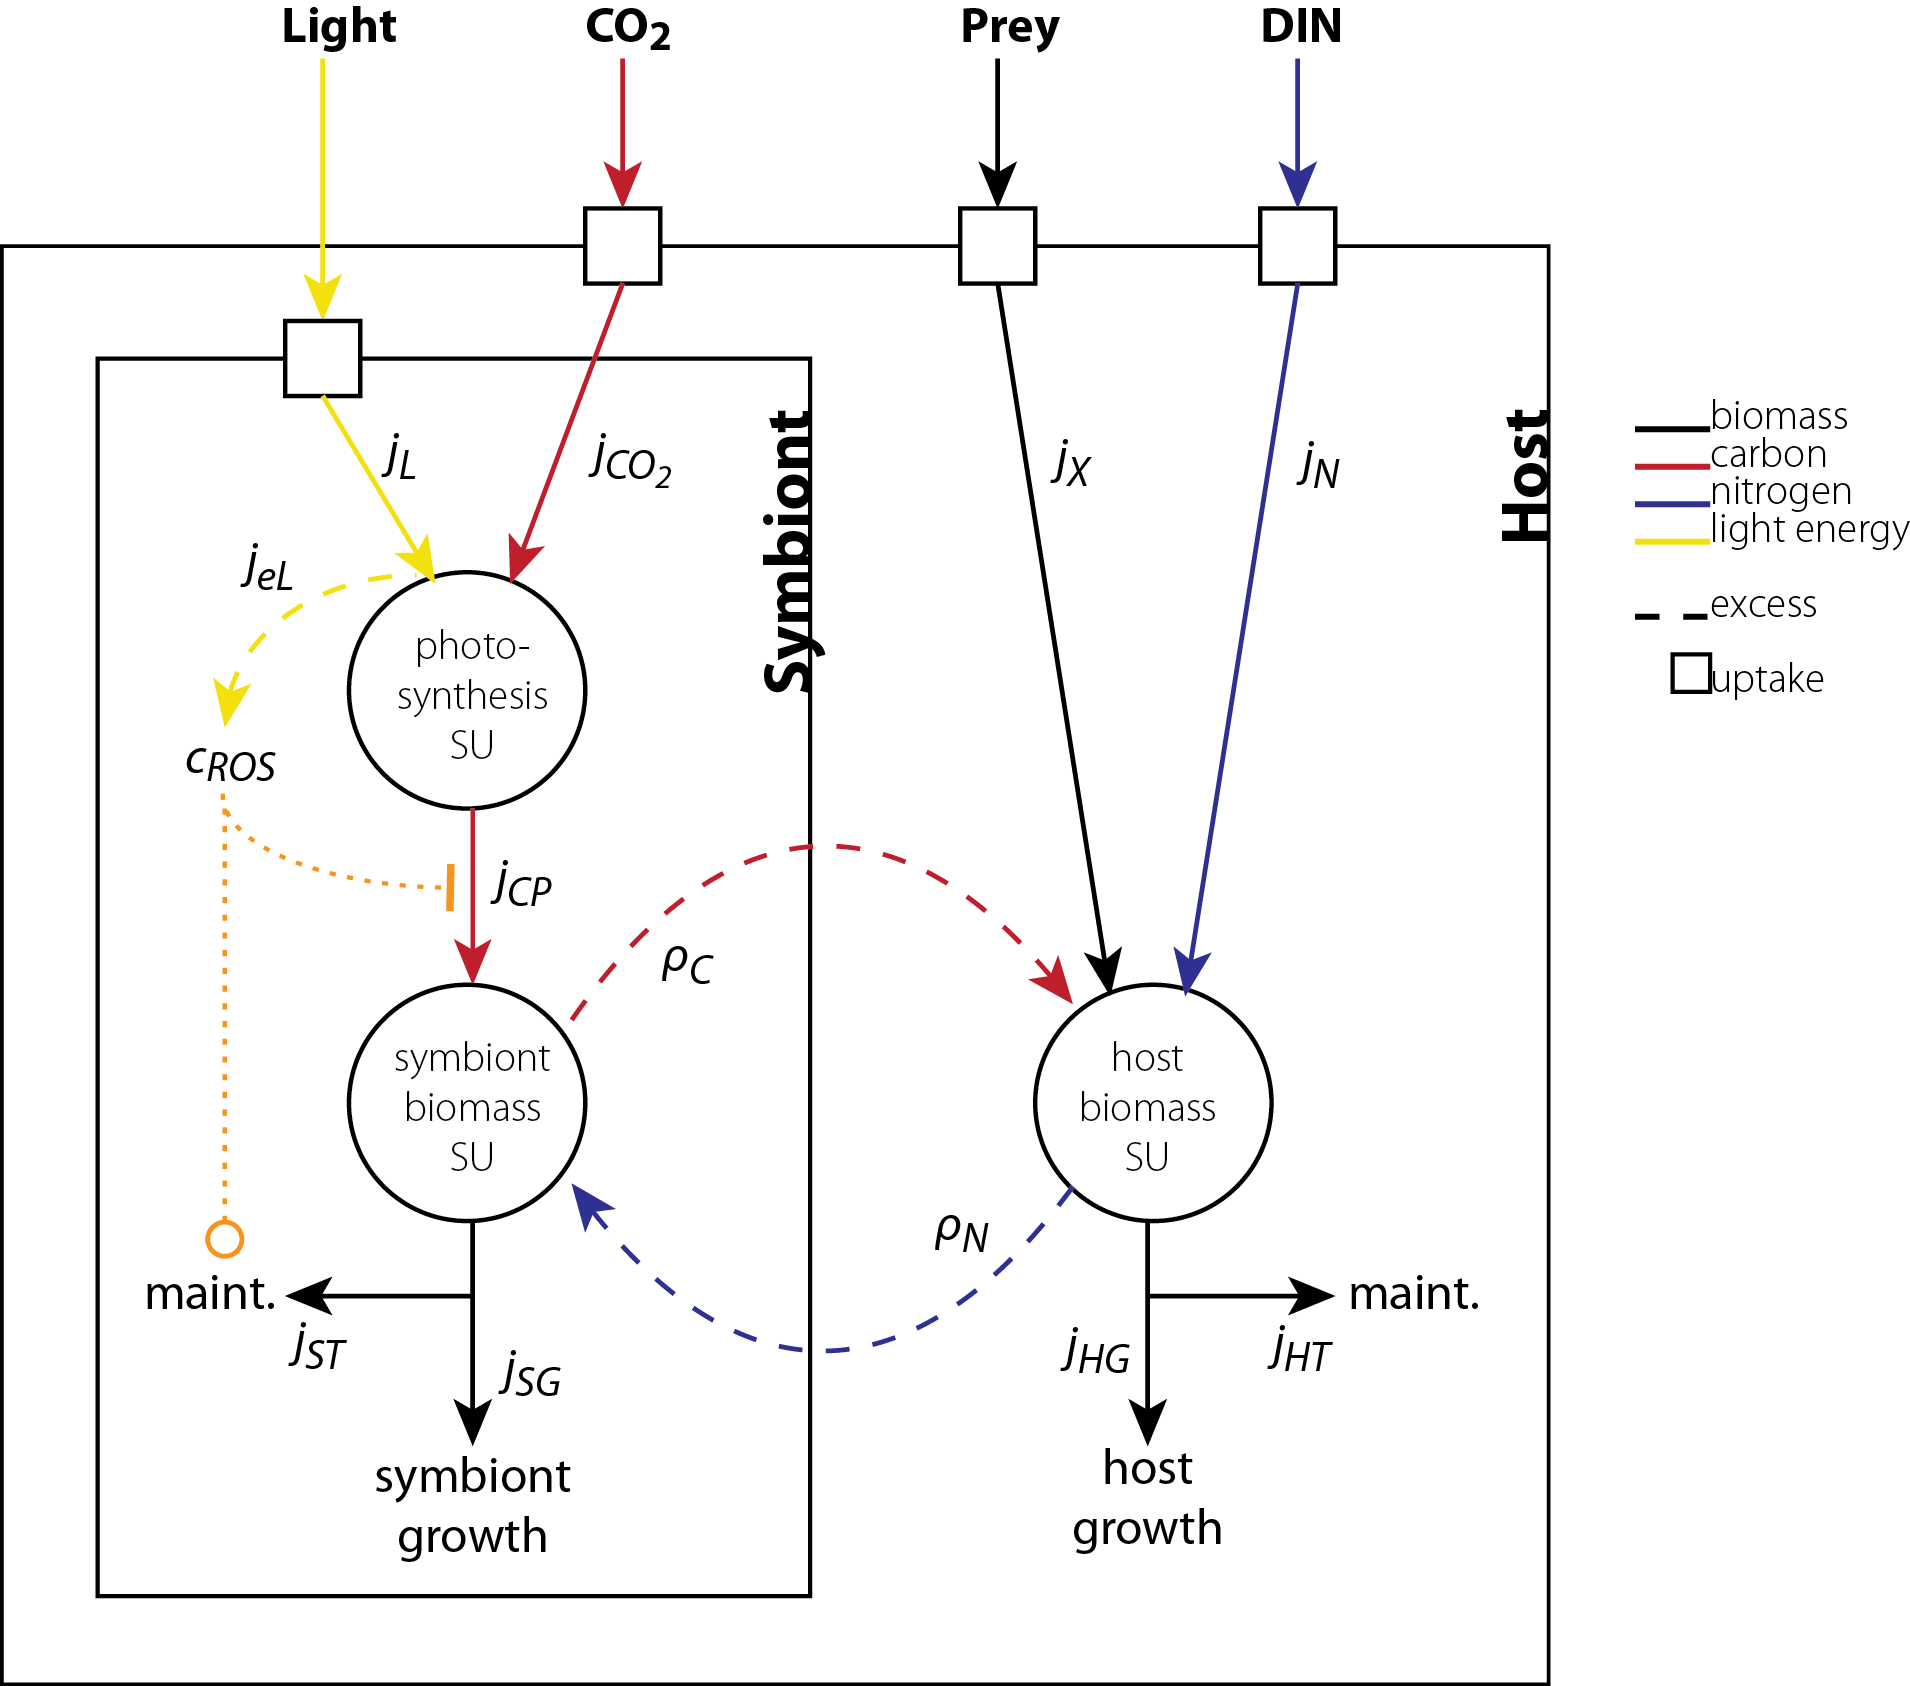
\includegraphics{../img/model.png}
\caption{Graphical representation of coral-algal symbiosis model.}
\end{figure}

\subsection{Coral animal fluxes}\label{coral-animal-fluxes}

The coral animal acquires both carbon and nitrogen from feeding on prey
from the environment. Prey acquisition is specified by Michaelis-Menten
kinetics using a maximum area-specific feeding rate and half-saturation
constant:

\begin{equation} j_X = {{j_{Xm} \cdot X} \over {X + K_X}} \end{equation}

Additionally, the coral animal can acquire nitrogen from the surrounding
seawater. This nitrogen source is assumed to represent ammonium, the
primary form utilized by corals (Wang and Douglas 1998; Yellowlees,
Rees, and Leggat 2008). The uptake of nitrogen from the environment is
specified by Michaelis-Menten kinetics using a maximum area-specific
uptake rate and half-saturation constant:

\begin{equation} j_N = {{j_{Nm} \cdot N} \over {N + K_N}} \end{equation}

Coral biomass formation is specified by a parallel complementary SU that
combines carbon and nitrogen to form biomass. In addition to the carbon
and nitrogen acquired by direct uptake (Eqs. 1 and 2), the coral
recycles a portion of the nitrogen liberated by biomass turnover
(\(r_{NH}=\sigma_{NH}j_{HT}^0\)), and receives surplus fixed carbon
shared by the symbiont (\(\rho_C\)), such that the total biomass
formation is specified as:

\begin{equation} j_{HG} = \bigg({1 \over j_{HGm}} + {1 \over {\rho_C{S \over H} + j_X}} + {1 \over {(j_N + n_{NX}j_X + r_{NH}) / n_{NH}}} - {1 \over {{\rho_C{S \over H} + j_X} + (j_N + n_{NX}j_X + r_{NH}) / n_{NH}}}\bigg)^{-1} \end{equation}

The amount of nitrogen input to the coral biomass SU in excess of what
is actually consumed in biomass formation (i.e., surplus nitrogen, or
the ``rejection flux'' in SU terminology) is then made available to the
symbiont, and is specified as:

\begin{equation} \rho_N = (j_N + n_{NX}j_X + r_{NH} - n_{NH}j_{HG})_+ \end{equation}

Due to the inherent inefficiency of the parallel complementary SU
formulation, there will always be some nitrogen shared with the symbiont
even when coral biomass formation is strongly nitrogen-limited.
Likewise, there is always a non-zero rejection flux of carbon from the
coral biomass SU, which is assumed to be lost to the environment.

\subsection{\texorpdfstring{\emph{Symbiodinium}
fluxes}{Symbiodinium fluxes}}\label{symbiodinium-fluxes}

The symbiont produces fixed carbon through photosynthesis, a process
represented here by a single SU with two substrates: light (photons) and
inorganic carbon (CO\textsubscript{2}). The amount of light absorbed by
the symbiont depends on the scalar irradiance at the site of light
absorption, which is modified substantially relative to external
downwelling irradiance owing to multiple scattering by the coral
skeleton and self-shading by surrounding symbionts (Enríquez, Méndez,
and Iglesias-Prieto 2005; Marcelino et al. 2013). We used data from
Marcelino et al. (2013) to empirically derive the ratio of internal
scalar irradiance to external downwelling irradiance as a function of
symbiont density (expressed as symbiont to host biomass ratio), and
subsequently multiply this quantity by the external downwelling
irradiance \(L\) and the effective light-absorbing surface area of
symbiont biomass \(ds\) to specify the amount of light absorbed:

\begin{equation} j_L = \big[1.26 + 1.39 \cdot \exp(-6.48 \cdot {S \over H})\big] \cdot L \cdot \bar{a}^* \end{equation}

We then specify two pathways for input of inorganic carbon to the
photosynthesis SU: 1) passive diffusion of CO\textsubscript{2} from the
external environment, and 2) active delivery of CO\textsubscript{2} to
the symbiont by the host. The passive flux ensures that some
CO\textsubscript{2} is always available to photosynthesis, and the
active flux encompasses the potentially diverse mechanisms by which the
host may enhance CO\textsubscript{2} availability for the symbiont,
including active transport of bicarbonate, carbonic anhydrase-catalyzed
conversion of bicarbonate to CO\textsubscript{2} to promote diffusion
toward the symbiont, and acidification of the symbiosome to increase
localized CO\textsubscript{2} concentrations. Since the host physically
separates the symbiont from the external environment, both the passive
and active flux rates are proportional to host surface area. A more
rigorous, mechanistic model of inorganic carbon processing would require
spatially explicit internal pools accounting for pH and carbon
speciation, which is beyond the current scope of this work. Instead, the
specification of CO\textsubscript{2} delivery rates offers the user the
opportunity to compare different rates of CO\textsubscript{2} delivery
that may characterize different coral species (Wooldridge 2014a). The
input of CO\textsubscript{2} to the photosynthesis SU is therefore
specified as:

\begin{equation} j_{CO_2} = j_{CO_2}^p + j_{CO_2}^a \end{equation}

In addition to the inputs CO\textsubscript{2} specified in Eqs. 7,
additional CO\textsubscript{2} representing the metabolic production of
CO\textsubscript{2} from host and symbiont biomass turnover
(\(r_{CH}=\sigma_{CH}j_{HT}^0; r_{CS}=\sigma_{CS}j_{ST}^0\)) is made
available to the photosynthesis SU. fixed carbon is produced by the
photosynthesis SU according to:

\begin{equation} j_{CP} = \bigg({1 \over j_{CPm}} + {1 \over {n_{LC} j_L }} + {1 \over {(j_{CO_2} + r_{CH}){H \over S} + r_{CS}}} - {1 \over {n_{LC} j_L + (j_{CO_2} + r_{CH}){H \over S} + r_{CS}}}\bigg)^{-1} \cdot c_{ROS}^{-1} \end{equation}

where \(j_{CPm}\) is the maximum specific rate of photosynthesis, and
\(c_{ROS}\) is the photooxidative stress multiplier (see below).
Dividing by \(c_{ROS}\) causes the rate of photosynthesis to decline in
response to photo-oxidative stress, a phenomenon known as
photoinhibition.

Light energy absorbed in excess of what is used to fix carbon is
specified by the SU ``rejection flux'', according to:

\begin{equation} j_{eL} = (j_L - j_{CP} / n_{LC})_+ \end{equation}

This excess light energy must be quenched by alternative pathways in
order to prevent photo-oxidative damage. \emph{Symbiodinium} may utilize
a variety of pathways for non-photochemical quenching (NPQ; Roth 2014),
which we collect in a total capacity for NPQ as a parameter of the
symbiont (\(j_{NPQ}\)). If light energy exceeds the total capacity of
both carbon fixation and NPQ, then damaging reactive oxygen species
(ROS) may be produced. We represent this as a scaled flux of ROS
\(c_{ROS}\), which takes a value of 1 when all light absorbed is
quenched by photochemistry and NPQ, and increases as the amount of
excess excitation energy increases.

\begin{equation} c_{ROS} = 1 + \bigg[\bigg({{j_{eL} - j_{NPQ}} \over k_{ROS}}\bigg)^k\bigg]_+ \end{equation}

where \(j_{NPQ}\), \(k_{ROS}\), and \(k\) are parameters of the symbiont
that determine the onset and rate of ROS production. Importantly,
\(c_{ROS}\) as specified here is not a function of absolute light
absorption, but rather the amount of excess light energy \(j_{eL}\)
after accounting for carbon fixation and NPQ. A direct consequence of
this formulation is that carbon-limitation of photosynthesis can lead to
photo-oxidative stress, a mechanism of biological importance (Wooldridge
2009) that was not captured by previous representations of
photo-oxidative stress (Eynaud, Nisbet, and Muller 2011). Moreover, this
formulation allows functional diversity among symbiont types to be
explored by changing the parameters \(j_{NPQ}\), \(k_{ROS}\), and \(k\).

Carbon fixed by photosynthesis (\(j_{CP}\)) is then used in conjunction
with nitrogen shared by the host (\(\rho_N\)) and a proportion of
nitrogen recycled from symbiont biomass turnover
(\(r_{NS}=\sigma_{NS}j_{ST}^0\)) to build new symbiont biomass,
following the SU equation:

\begin{equation} j_{SG} = \bigg({1 \over j_{SGm}} + {1 \over j_{CP}} + {1 \over {(\rho_N{H \over S} + r_{NS}) / n_{NH}}} - {1 \over {j_{CP} + (\rho_N{H \over S} + r_{NS}) / n_{NH}}}\bigg)^{-1} \end{equation}

The rejection flux of carbon from this SU represents the amount of fixed
carbon produced by photosynthesis in excess of what can be used to
produce symbiont biomass; this surplus \(\rho_C\) is translocated to the
coral host:

\begin{equation} \rho_C = (j_{CP} - j_{SG})_+ \end{equation}

The rejection flux of nitrogen from the symbiont biomass SU is lost to
the environment.

Symbiont biomass turnover includes a component of constant turnover
specified by the parameter \(j_{ST}^0\), representing fixed maintenance
costs, plus a component that scales with the magnitude of ROS
production.

\begin{equation} j_{ST} = j_{ST}^0(1 + 5 \cdot (c_{ROS}-1)) \end{equation}

This second component of symbiont biomass loss can represent both
photodamage and/or symbiont expulsion (i.e., bleaching), both of which
happen in response to higher levels or ROS production. The constant 5 is
included to increase biomass loss in response to ROS. (Note that
recycling of symbiont biomass turnover (\(rNS\) and \(rCS\)) only occurs
based on the basal maintenance related turnover (i.e., \(j_{ST}^0\)),
and not the bleaching-related biomass loss, as this loss represents
biomass being damaged or being expelled from the holobiont).

\subsection{Model state equations}\label{model-state-equations}

Finally, the balance equations representing the specific growth rates of
symbiont and host biomass over time can be expressed as:

\begin{equation} {dS \over Sdt} = j_{SG} - j_{ST} \end{equation}

\begin{equation} {dH \over Hdt} = j_{HG} - j_{HT}^0 \end{equation}

\subsection{Numerical analysis}\label{numerical-analysis}

A time-stepping Euler method was used to solve the state equations since
the production and rejection fluxes of the SUs are imiplicitly defined.
Specifically, the rejection fluxes of carbon and nitrogen from the
symbiont and host biomass SUs act as reciprocal input fluxes to the
other SU. In addition, the rejection flux of excitation energy from the
photosynthesis SU acts to reduce its own production flux (i.e.,
photoinhibition), and hence a discretized time-stepping procedure was
necessary. A vector of time values was created for each simulation run,
along which dynamic environmental forcing functions (irradiance, DIN,
and prey abundance) can be designed. These vectors, along with initial
values of symbiont and host biomass, then serve as input to the
time-stepping function, which solves for the current system state using
values of the previous system state where necessary. A default time step
of 0.1 days was used for all simulations, which were performed using R
code that is available in the data repository accompanying this article:
\url{github.com/jrcunning/Rcoral}.

\section{Model behavior evaluation}\label{model-behavior-evaluation}

To analyze qualitative behavior, we ran the model to steady state across
gradients of external irradiance and DIN, and plotted the specific
growth rate (Fig. 2A) and symbiont to host biomass ratio (Fig. 2B).
Results are consistent with observations in corals: specific growth
rates are low at very low levels of irradiance and DIN, as these
scenarios limit the availability of carbon and nitrogen, respectively,
to build biomass. As these resources increase, specific growth
increases, reaching its highest levels above 2 µM DIN and
\textasciitilde{}15 mol photons m\textsuperscript{-2}
d\textsuperscript{-1}.

\begin{figure}[htbp]
\centering
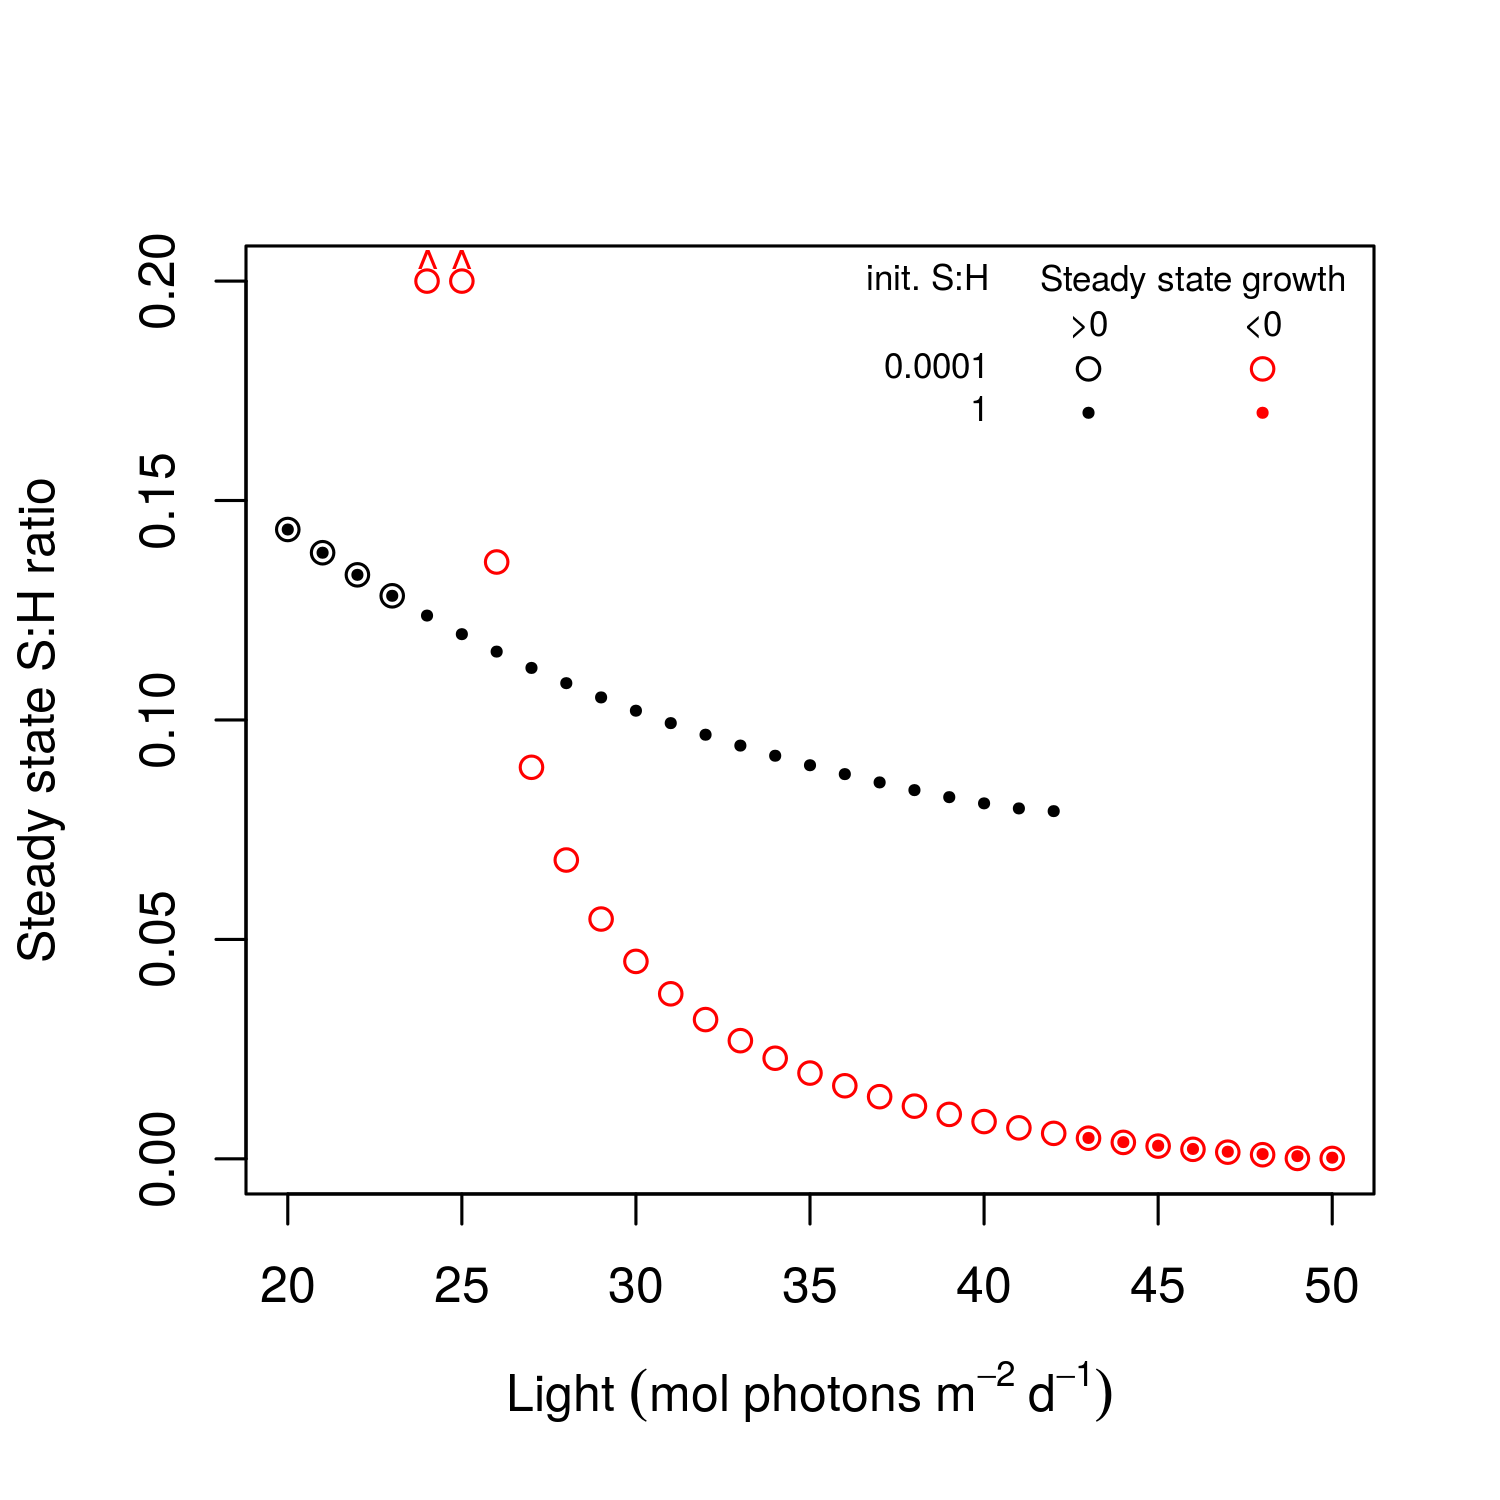
\includegraphics{../img/Fig2.png}
\caption{Steady state values of (A) specific growth (\$Cmol
Cmol\textsuperscript{-1} d\textsuperscript{-1}) and (B) the symbiont to
host biomass ratio (CmolS CmolH\textsuperscript{-1}) across gradients of
external irradiance and dissolved inorganic nitrogen. Simulations for
each combination of light and nutrients (21 points along each axis) were
run for 100 days with a time step of 1 day. Negative steady state growth
rates, and corresponding S:H ratios, were set to zero.}
\end{figure}

\section{Discussion - Potential
applications/utility}\label{discussion---potential-applicationsutility}

\section*{References}\label{references}
\addcontentsline{toc}{section}{References}

\hypertarget{refs}{}
\hypertarget{ref-Costanza:2014ex}{}
Costanza, R, R de Groot, and P Sutton. 2014. ``Changes in the global
value of ecosystem services.'' \emph{Global Environmental \ldots{}} 26:
152--58.
doi:\href{https://doi.org/10.1016/j.gloenvcha.2014.04.002}{10.1016/j.gloenvcha.2014.04.002}.

\hypertarget{ref-Enriquez:2005p142}{}
Enríquez, Susana, Eugenio R Méndez, and Roberto Iglesias-Prieto. 2005.
``Multiple scattering on coral skeletons enhances light absorption by
symbiotic algae.'' \emph{Limnology and Oceanography} 50 (4): 1025--32.

\hypertarget{ref-Eynaud:2011tv}{}
Eynaud, Yoan, Roger M Nisbet, and Erik B Muller. 2011. ``Impact of
excess and harmful radiation on energy budgets in scleractinian
corals.'' \emph{Ecological Modelling} 222 (7). Elsevier: 1315--22.
\url{http://www.sciencedirect.com/science/article/pii/S0304380011000263}.

\hypertarget{ref-Glynn:2001p7571}{}
Glynn, Peter W, Juan L Maté, Andrew C Baker, and MO Calderón. 2001.
``Coral bleaching and mortality in Panama and Ecuador during the
1997-1998 El Niño-Southern Oscillation event: Spatial/temporal patterns
and comparisons with the 1982-1983 event.'' \emph{Bulletin of Marine
Science} 69 (1): 79--109.
\url{http://www.scopus.com/record/display.url?fedsrfIntegrator=MEKPAPERS-SCOCIT\&origin=fedsrf\&view=basic\&eid=2-s2.0-0034761826}.

\hypertarget{ref-Jager:2013bj}{}
Jager, Tjalling, Benjamin T Martin, and Elke I Zimmer. 2013. ``DEBkiss
or the quest for the simplest generic model of animal life history.''
\emph{Journal of Theoretical Biology} 328: 9--18.
doi:\href{https://doi.org/10.1016/j.jtbi.2013.03.011}{10.1016/j.jtbi.2013.03.011}.

\hypertarget{ref-Jokiel:1977p7353}{}
Jokiel, Paul L, and SL Coles. 1977. ``Effects of temperature on the
mortality and growth of Hawaiian reef corals.'' \emph{Marine Biology} 43
(3): 201--8.
\url{http://www.scopus.com/record/display.url?fedsrfIntegrator=MEKPAPERS-SCOCIT\&origin=fedsrf\&view=basic\&eid=2-s2.0-0000237488}.

\hypertarget{ref-Kooijman:2010vd}{}
Kooijman, SALM. 2010. \emph{Dynamic Energy Budget Theory for Metabolic
Organization}. 3rd ed. Cambridge University Press.

\hypertarget{ref-Marcelino:2013hz}{}
Marcelino, Luisa A, Mark W Westneat, Valentina Stoyneva, Jillian Henss,
Jeremy D Rogers, Andrew Radosevich, Vladimir Turzhitsky, et al. 2013.
``Modulation of Light-Enhancement to Symbiotic Algae by Light-Scattering
in Corals and Evolutionary Trends in Bleaching.'' \emph{PLoS ONE} 8 (4):
e61492.
doi:\href{https://doi.org/10.1371/journal.pone.0061492.s008}{10.1371/journal.pone.0061492.s008}.

\hypertarget{ref-Muller:2009io}{}
Muller, Erik B, Sebastiaan A L M Kooijman, Peter J Edmunds, Francis J
Doyle, and Roger M Nisbet. 2009. ``Dynamic energy budgets in syntrophic
symbiotic relationships between heterotrophic hosts and photoautotrophic
symbionts.'' \emph{Journal of Theoretical Biology} 259 (1): 44--57.
doi:\href{https://doi.org/10.1016/j.jtbi.2009.03.004}{10.1016/j.jtbi.2009.03.004}.

\hypertarget{ref-Muscatine:1977p4220}{}
Muscatine, Leonard, and James W Porter. 1977. ``Reef corals: mutualistic
symbioses adapted to nutrient-poor environments.'' \emph{Bioscience} 27
(7): 454--60.

\hypertarget{ref-RALanguageandEn:2014wf}{}
R Core Team. 2014. ``R: A Language and Environment for Statistical
Computing.'' Vienna, Austria: R Foundation for Statistical Computing.
\url{http://www.R-project.org/}.

\hypertarget{ref-Roth:2014wf}{}
Roth, M S. 2014. ``The engine of the reef: Photobiology of the
coral-algal symbiosis.'' \emph{Frontiers in Microbiology}.
\url{http://journal.frontiersin.org/Journal/10.3389/fmicb.2014.00422/pdf}.

\hypertarget{ref-Wang:1998p128}{}
Wang, J, and Angela E Douglas. 1998. ``Nitrogen recycling or nitrogen
conservation in an alga-invertebrate symbiosis?'' \emph{The Journal of
Experimental Biology} 201: 2445--53.

\hypertarget{ref-Weis:2008p944}{}
Weis, Virginia M. 2008. ``Cellular mechanisms of Cnidarian bleaching:
stress causes the collapse of symbiosis.'' \emph{The Journal of
Experimental Biology} 211 (Pt 19): 3059--66.
doi:\href{https://doi.org/10.1242/jeb.009597}{10.1242/jeb.009597}.

\hypertarget{ref-Wooldridge:2009p7807}{}
Wooldridge, Scott A. 2009. ``A new conceptual model for the warm-water
breakdown of the coral-algae endosymbiosis.'' \emph{Marine and
Freshwater Research} 60 (June): 483--96.

\hypertarget{ref-Wooldridge:2014di}{}
---------. 2014a. ``Differential thermal bleaching susceptibilities
amongst coral taxa: re-posing the role of the host.'' \emph{Coral Reefs}
33 (1). Springer Berlin Heidelberg: 15--27.
doi:\href{https://doi.org/10.1007/s00338-013-1111-4}{10.1007/s00338-013-1111-4}.

\hypertarget{ref-Wooldridge:2014hc}{}
---------. 2014b. ``Formalising a mechanistic linkage between
heterotrophic feeding and thermal bleaching resistance.'' \emph{Coral
Reefs}. Springer Berlin Heidelberg, 1--6.
doi:\href{https://doi.org/10.1007/s00338-014-1193-7}{10.1007/s00338-014-1193-7}.

\hypertarget{ref-Yellowlees:2008p331}{}
Yellowlees, David, T A V Rees, and William Leggat. 2008. ``Metabolic
interactions between algal symbionts and invertebrate hosts.''
\emph{Plant, Cell and Environment} 31: 679--94.

\end{document}


